The kinematics of human gaze motion are determined by the anatomic and neurophysiological properties of the human visuomotor system. These properties include eye dimensions (human eyes are approximately 2.5 $cm$ wide), inter-eye distance (mean interpupillary distance is approximately 6.4 cm), and ocular motor range (in humans, OMR is radially symmetric and ranges from 45$^\circ$ to 55$^\circ$.) Stylized characters often have much larger eyes, greater inter-eye spacing, and their stylized shape mandates a narrow and often asymmetric OMR. When human gaze shift movements are applied to such stylized characters, we observe two kinds of phenomena. First, anatomically correct, but rarely observed, elements of human gaze can be magnified and become noticeable. Second, asymmetry and exaggerated size of the eyes can cause anomalous situations that are rare or impossible in healthy human gaze. We argue that these phenomena are undesirable, as they can distract the viewer and alter the meaning of the gaze shift. Below, we catalog specific visual artifacts that our methods seek to address.

\emph{Cross-eyedness} occurs when the eyes significantly angle inward (towards each other). In humans, the eyes must angle toward each other to fixate a target. However, excessive inward angling of the eyes is straining to maintain, as one can verify by fixating a target at a very small proximity, e.g., the tip of one's nose. Small amounts of cross-eyedness are not noticeable due to the small eye size and inter-eye distance, while larger amounts are caused by unnatural viewing conditions or an explicit expression. In characters with large or widely spaced eyes, cross-eyedness becomes noticeable even in more standard viewing (Figure~\ref{fig:CrosseyednessFixExample}).

\emph{Speedy eyes} are implausibly fast eye movements in characters with large eyes. Human eyes have low mass and strong muscles that support fast and abrupt movements in excess of 400$^\circ/s$, but such rapid movements can appear implausible in stylized characters.

\emph{OMR-block} occurs when the character's eyes reach the boundary of the OMR and are unable to move until the head brings them into alignment with the gaze target. While natural and common in humans, this phenomenon can appear anomalous in stylized characters; during this prolonged phase when the eyes are stationary, the character may appear static and puppet-like. We believe this phenomenon to be caused by \textit{speedy eyes}; the eyes cover the distance between starting position and the OMR at an unrealistic speed, resulting in an unusually long period of OMR-block. The visual artifact becomes even more prevalent with a narrow OMR, a common property of stylized characters.

\begin{figure}
\centering
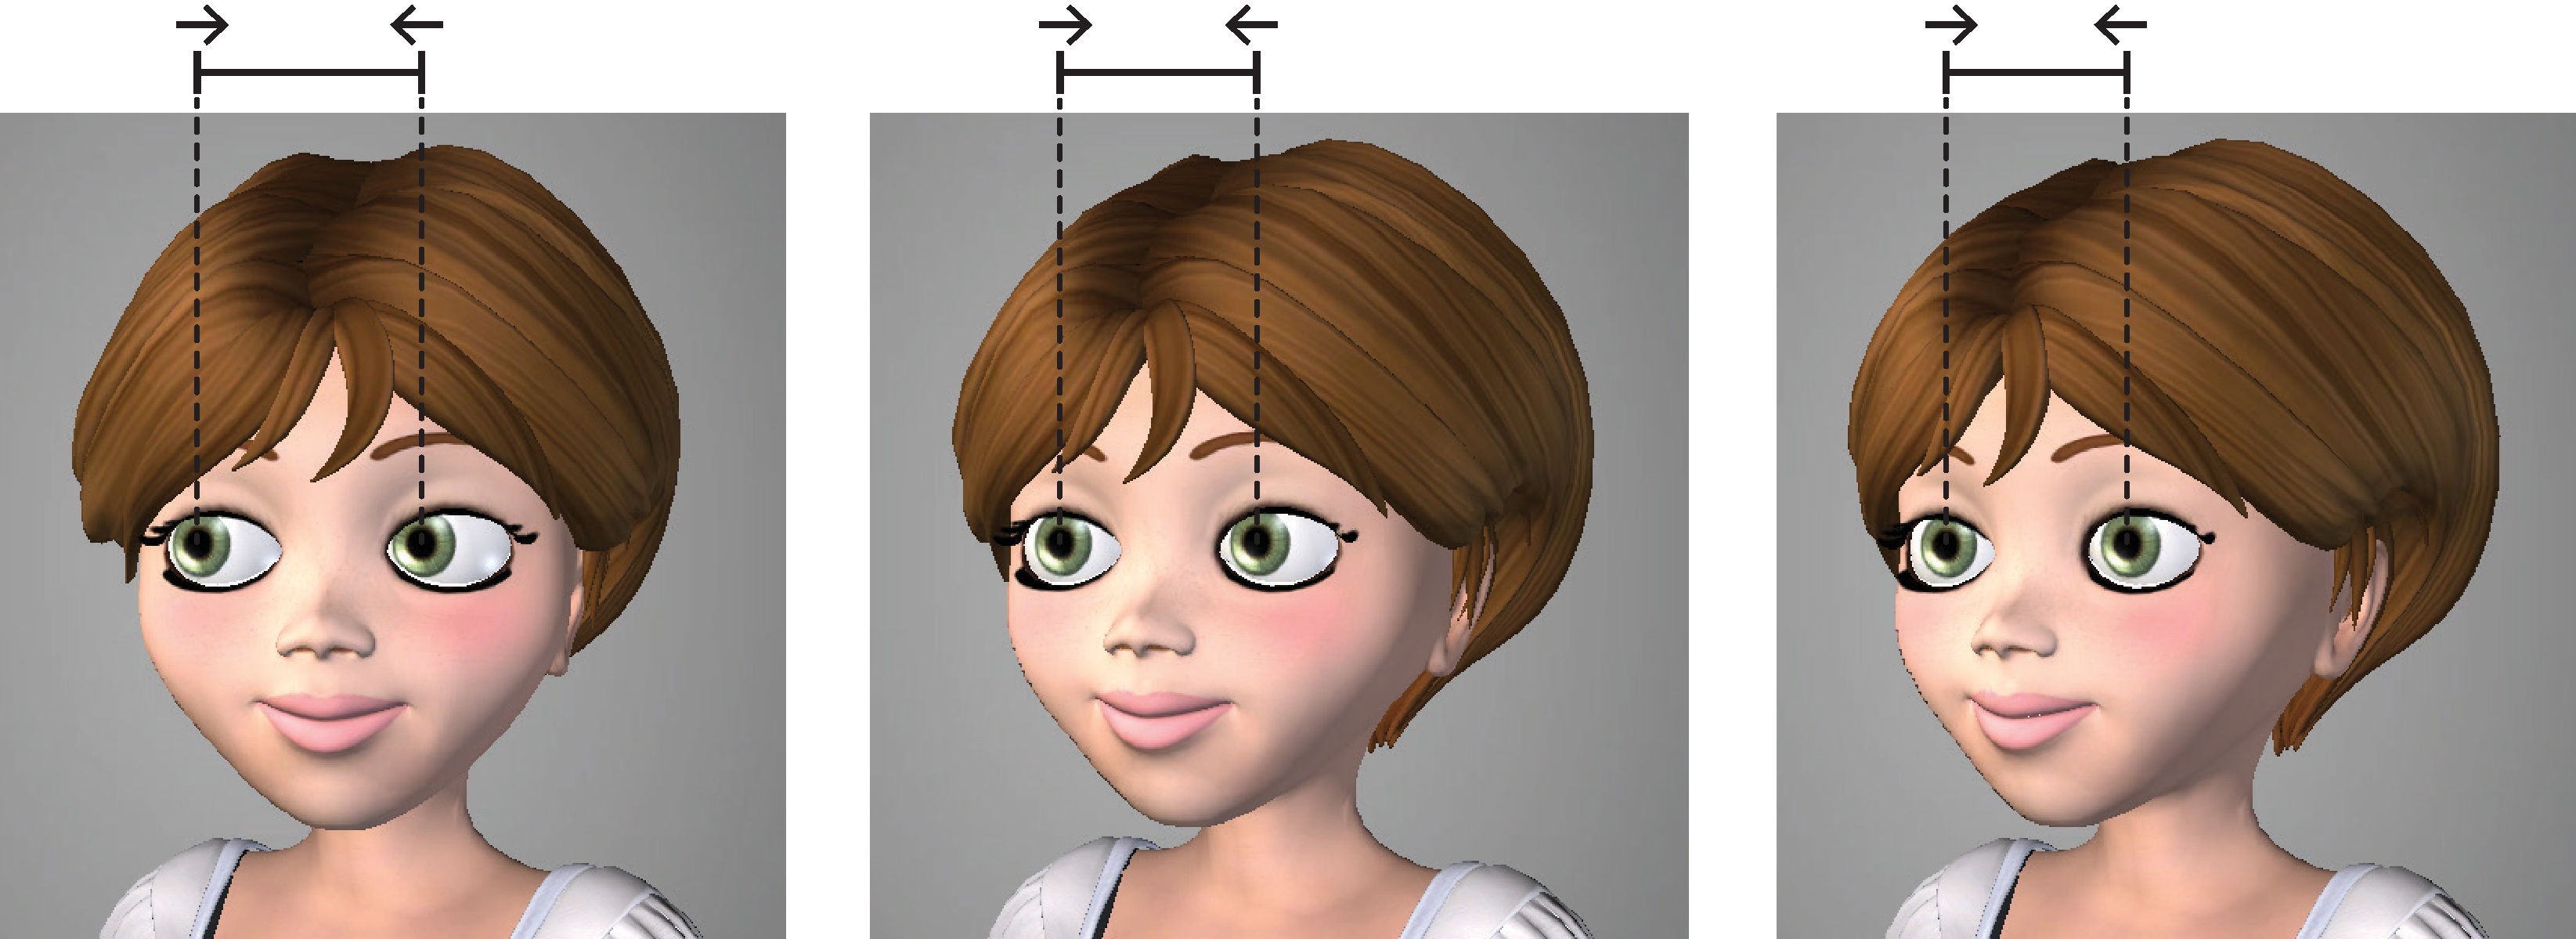
\includegraphics[width=0.85\textwidth]{stylizedgaze/Figures/EyeRetractionExample-small.pdf}
\caption{Eye retraction example. The right eye has aligned with the target and is retracting as the left eye moves forward. Notation: Solid line indicates inter-eye distance. Arrows $\rightarrow$ and $\leftarrow$ indicate eye movement directions.}
\label{fig:EyeRetractionExample}
\end{figure}

\emph{Eye retraction} occurs when the head brings the eyes into alignment with the gaze target and the \textit{vestibulo-ocular reflex} (VOR) locks the eyes onto the target as the head catches up, rotating the eyes in the opposite direction of the head movement. While this does not appear as anomalous in real human gaze or characters with humanlike proportions, in stylized characters with large eyes, it can appear as if the eyes have overshot the target and are now retracting in order to realign with it (Figure~\ref{fig:EyeRetractionExample}). We believe that the cause of this illusion is in excessive eye velocities that cause the eyes to advance further ahead and retract more than expected.

\begin{figure}
\centering
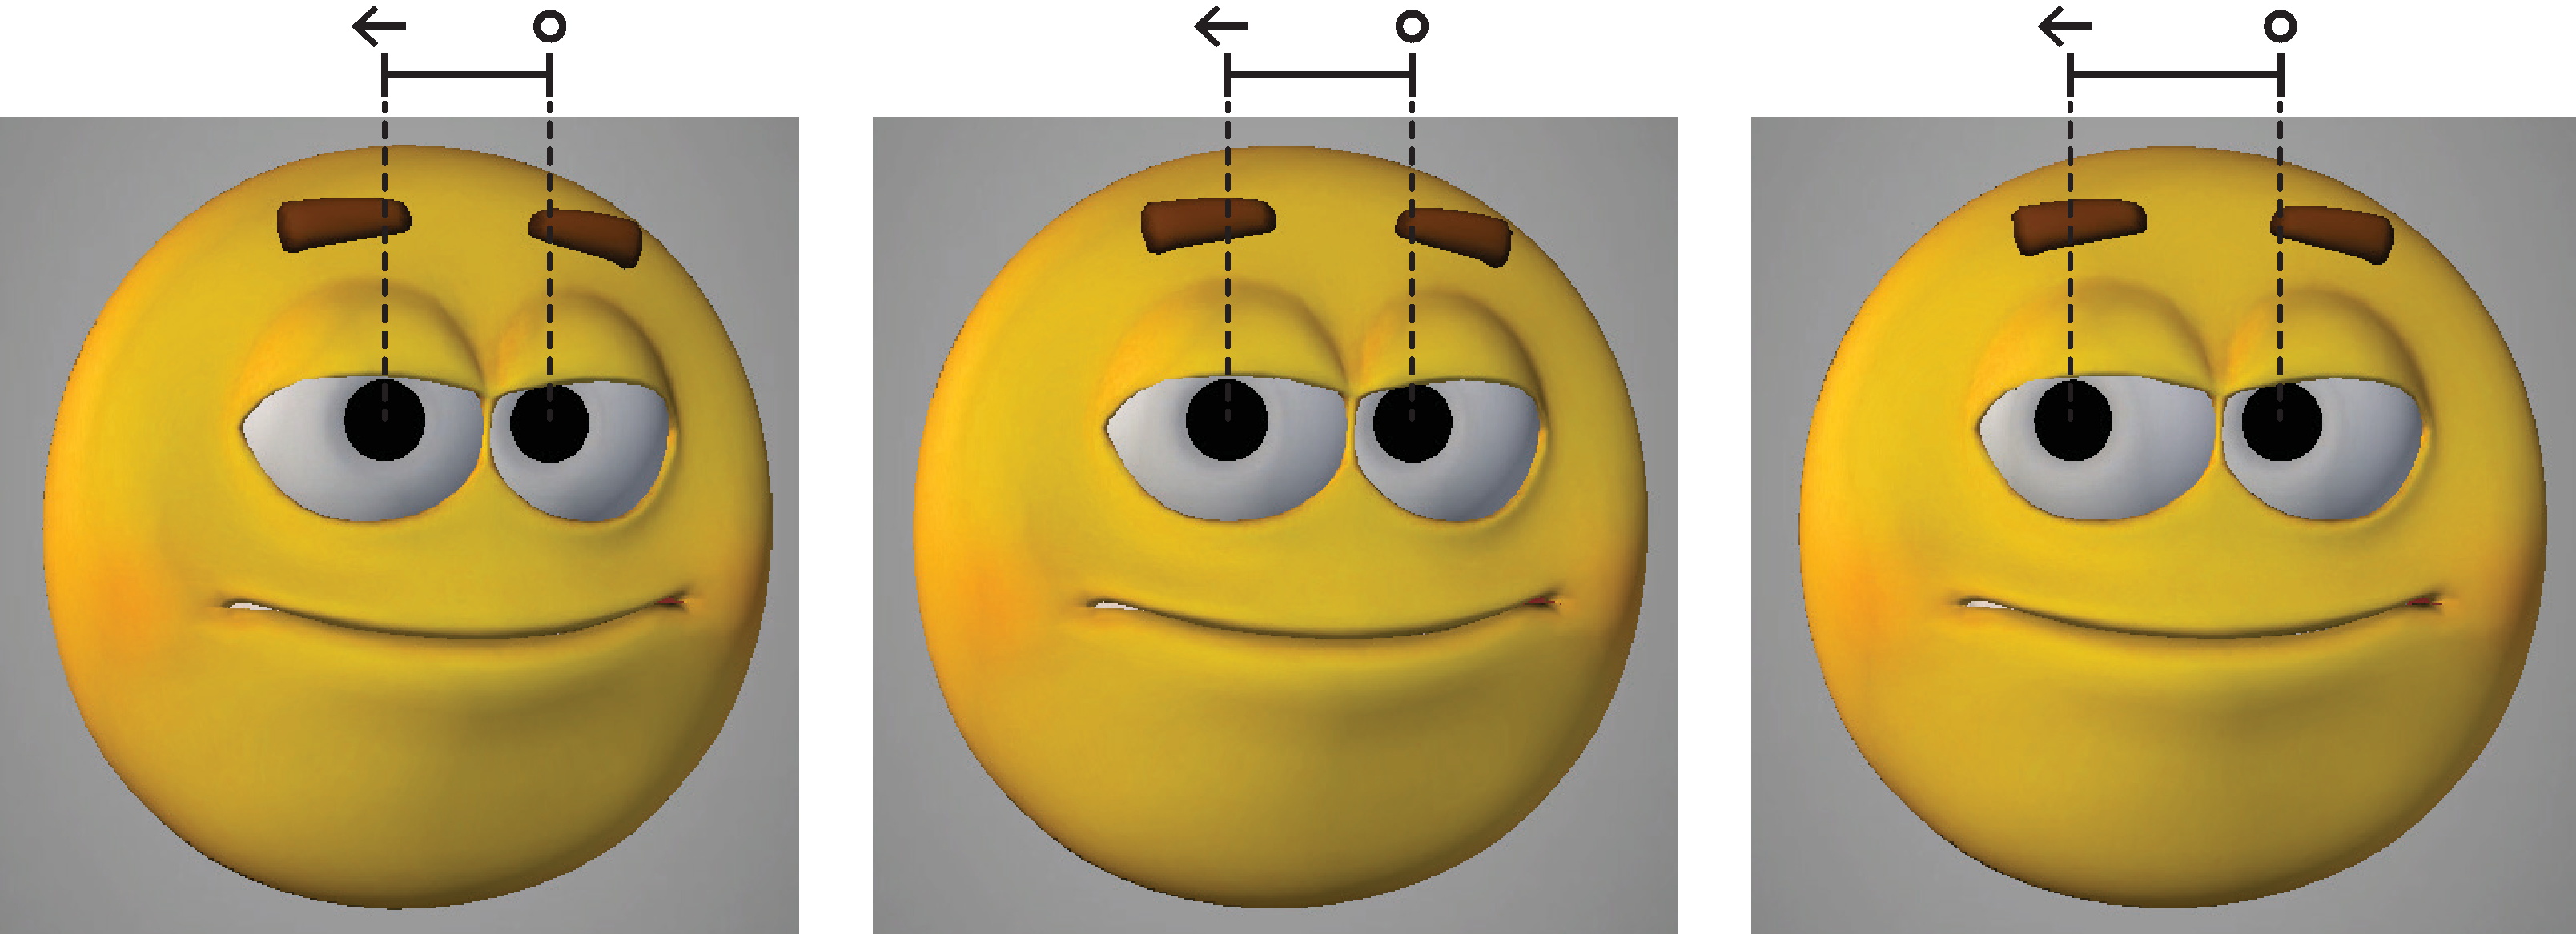
\includegraphics[width=0.85\textwidth]{stylizedgaze/Figures/StuckEyeExample-small.pdf}
\caption{Stuck eye example. The right eye is moving ahead, while the left eye is blocked by the OMR. Notation: Dot $\circ$ indicates that the eye is stationary.}
\label{fig:StuckEyeExample}
\end{figure}

\emph{Stuck eye} is caused by the asymmetry of eye shape, which necessarily involves asymmetry in the OMR. The leading eye in the gaze shift, which rotates outward, has a greater distance to cover before reaching the OMR than the trailing eye. However, when both eyes move at the same velocity, as is the case with human eyes, the trailing eye will reach its OMR boundary sooner and become blocked, while the other eye will continue moving (Figure~\ref{fig:StuckEyeExample}). Movement in only one eye does not occur in human gaze except in medical conditions such as amblyopia and therefore can appear abnormal.

\emph{Eye divergence} occurs when the eyes have asymmetric OMR. In such cases, eye gaze directions can become divergent as they reach their respective OMR boundaries. Although difficult to observe in static poses, this divergence causes disconjugate eye movements and appears jarring when the eyes are brought into alignment with the gaze target. In these movements, the leading eye reaches the gaze target before the trailing eye, and VOR causes the eye to rotate backward, while the trailing eye is still moving forward (Figure~\ref{fig:EyeDivergenceFixExample}). Such divergent orientations and disconjugate movements are improbable in healthy human gaze and appear anomalous. 